\documentclass{article}


\usepackage{arxiv}

\usepackage[utf8]{inputenc} % allow utf-8 input
\usepackage[T1]{fontenc}    % use 8-bit T1 fonts
\usepackage{hyperref}       % hyperlinks
\usepackage{url}            % simple URL typesetting
\usepackage{booktabs}       % professional-quality tables
\usepackage{amsfonts}       % blackboard math symbols
\usepackage{nicefrac}       % compact symbols for 1/2, etc.
\usepackage{microtype}      % microtypography
\usepackage{lipsum}
\usepackage{fancyhdr}       % header
\usepackage{graphicx}       % graphics
\graphicspath{{figures/}}     % organize your images and other figures under figures/ folder
\usepackage{tikz}
\usepackage{tabularx}
\usepackage{array}
% \usepackage{natbib}
\PassOptionsToPackage{numbers, compress}{natbib}


\newcommand{\halfcircle}{
  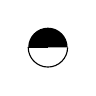
\begin{tikzpicture}[baseline=-0.75ex]
    \fill[black] (0,0) -- (0.25,0) arc (0:180:0.25) -- cycle; % Fill the upper half
    \draw (0,0) -- (-0.25,0) arc (0:180:-0.25); % Draw the border for the lower half
  \end{tikzpicture}
}

%Header
\pagestyle{fancy}
\thispagestyle{empty}
\rhead{ \textit{ }} 

%% Title
% \halfcircle{}
\title{Open-Creator: Bridging Code Interpreter and Skill Library}

\author{
Junmin Gong\(^{*}\) \\
\texttt{gongjunmin@timedomain.ai} \\
Timedomain \\
\and
Sen Wang \(\dagger\) \\
\texttt{sayo@timedomain.ai} \\
Timedomain \\
\and
Wenxiao Zhao \(\dagger\) \\
\texttt{sean.z@timedomain.ai} \\
Timedomain \\
\and
Jing Guo\(\ddagger\) \\
\texttt{joe.g@timedomain.ai} \\
Timedomain \\
}


\begin{document}
\textcolor{red}{\textbf{Note:} The experimental section is currently in progress and will be updated in the subsequent versions.}
\maketitle
\begin{abstract}
AI agents enhanced with tools, particularly code interpreters, hold promising prospects for broad and deep applications. However, existing systems often require reinterpreting problems and generating new codes for similar tasks, rather than reusing previously written and validated functions, leading to inefficiencies in token usage and lack of generalization. In response to these challenges, we introduce \textit{open-creator}, a novel AI agents framework bridging code interpreters and skill libraries. Open-creator is designed to standardize various inputs (including, but not limited to, dialogic problem-solving experiences, code files, and API documentation) into a uniform skill object format. This framework supports local saving, searching, and cloud uploading by users. Adopting a modular strategy, open-creator allows developers and researchers to create, share, and reuse skills without concerns over compatibility or version control. Furthermore, it offers flexibility in modifying, assembling, and disassembling created skills, which is crucial as skills may need updates over time and with changing environments. This mechanism allows AI agents to continually optimize skills based on feedback and new data. Our approach paves the way for more efficient and adaptable AI agent functionalities, contributing to the field's ongoing development. The open-creator code is publicly accessible at: \href{https://github.com/timedomain-tech/open-creator}{https://github.com/timedomain-tech/open-creator}.
\end{abstract}

\section{Introduction}
AI agents engage in complex reasoning by integrating planning ~\cite{wei2022chain, xu2023rewoo, wang2023selfconsistency, yao2023tree}, decision-making, and the utilization of appropriate tools or APIs ~\cite{schick2023toolformer, li2023apibank}. However, these tools are typically predetermined and designed by humans, and the number of available tools is often limited due to the constraints on the input context length of Large Language Models (LLMs). To enhance the versatility of AI agents, a viable approach is to amalgamate the code-generation capabilities of LLMs with code execution functionalities. This integration allows for the flexible writing and execution of code to address specific user needs, embodying the role of Code Interpreters ~\cite{openinterpreter}.

Given that LLMs occasionally generate erroneous codes—leading to low robustness and inability to meet user requirements—recent research has focused on enabling LLMs to auto-correct codes through environmental feedback ~\cite{skreta2023errors, yao2022react, wang2023voyager, song2023llmplanner}. Additionally, there is emphasis on developing sophisticated projects through rational task decomposition and persistent memory. This focus has given rise to a plethora of AI agent frameworks, including MetaGPT ~\cite{hong2023metagpt}, ChatDev ~\cite{qian2023communicative}, GPT-enginger ~\cite{GPTEngineer}, GPT-term ~\cite{GPTeam}, and codeplan ~\cite{bairi2023codeplan}. These studies explore collaborative mechanisms among different roles, introduction of improved environments, enhanced feedback from agents, optimized task decomposition, and various engineering tricks, collectively contributing to the flourishing ecosystem of AI agents in the fields of Computer Science and Software Engineering. A comprehensive literature review in this area has been conducted by Wang et al ~\cite{wang2023survey}.

\begin{table}
\label{tab:learning_approaches}
\begin{tabularx}{\textwidth}{|c|>{\centering\arraybackslash}m{3cm}|>{\centering\arraybackslash}m{4cm}|>{\centering\arraybackslash}m{4cm}|c|}
\hline
 & \textbf{Learning} & \textbf{Outcome} & \textbf{Generalization} & \textbf{Interpretability} \\ \hline
ANN & Parameter Optimization & Weights of NN & Mapping Function & Low \\ \hline
LLM & Instruction Fine-tuning & Instruction-based LLM & In-context Learning Prompt & Medium \\ \hline
Agents & Tool Creation & Skill Library & RAG & High \\ \hline
\end{tabularx}
\centering
\vspace{2mm} % Adjust the space as you need
\caption{Comparison of Different Learning Approaches}
\end{table}

\section{Related Work}

Among the various contributions, two works, namely CREATOR ~\cite{qian2023creator} and VOYAGER ~\cite{wang2023voyager}, merit particular attention.

\subsection{CREATOR}

The CREATOR framework emerges as a noteworthy initiative addressing the intricate challenges faced by LLMs in tool utilization for problem-solving. Unlike conventional approaches, CREATOR uniquely positions LLMs not merely as users but as creators of tools. This pivotal transition enhances the models’ capabilities in solving problems with heightened precision and flexibility, offering a fresh perspective on leveraging the tool-creating prowess of LLMs. The framework comprises four stages:
\begin{itemize}
    \item \textbf{Creation:} LLMs are given explicit instructions and examples, guiding them to generate tools specific for given problems with focus on essential features.
    \item \textbf{Decision:} Post-tool creation, LLMs decide on tool application based on documentation and context analysis.
    \item \textbf{Execution:} This involves integrating the crafted tool code with the decision-making code, executing it through a code interpreter, and capturing the results or error messages.
    \item \textbf{Correction:} In case of execution failure, LLMs make necessary adjustments to the tool or decision, based on error tracking information.
\end{itemize}

The innovative approach of CREATOR brings to the forefront several advantages. Firstly, it alleviates the cognitive load on LLMs by distinctly separating the processes of abstract thinking (required for tool creation) and concrete thinking (necessary for decision-making). Secondly, the approach facilitates automated corrections through the strategic use of code testing and sensitivity analysis. Lastly, compared to LLM cache benefits ~\cite{GPTCache}, the validated tools crafted through CREATOR inherently possess superior generalization capabilities, making them adept at tackling a variety of new problems efficiently.

We consider the above as a new novel learning mechanism distinct from both the supervised learning in Artificial Neural Networks (ANNs) ~\cite{Schmidhuber_2015} and the few-shot in-context learning observed in LLMs ~\cite{dong2023survey}. Table~\ref{tab:learning_approaches} provides a concise summary of this proposition:

\begin{itemize}
    \item For ANNs, the traditional approach involves learning weights through gradient descent algorithms to approximate an input-output mapping function. The generalization capability of ANNs primarily relies on the quality of the supervised data and the efficacy of the mapping function itself.
    \item In the case of LLMs, extensive pre-training on large corpora coupled with fine-tuning through specific instructions allows these models to significantly improve performance on downstream tasks, even with only a few examples for in-context learning.
    \item Regarding Agents, the learning process transitions into a procedure where the interaction experiences with users, which are aimed at problem-solving, are converted into persistent skills. Generalization, in this context, involves utilizing Retrieval-Augmented Generation (RAG) ~\cite{lewis2021retrievalaugmented, li2022survey, mialon2023augmented} to semantically search and select the most appropriate tools for the current context, as well as handling parameter passing effectively.
\end{itemize}

This \textit{create and reuse} mechanism propels AI agents forward, capturing skills developed through LLMs. Unlike traditional deep learning, which often acts as a 'black box', this approach ensures skills are both reliable and interpretable. These skills are systematically stored in a library. When faced with new challenges, the system uses RAG techniques to select the best tools from this library. If no existing skill suffices, the system iteratively crafts new ones, ensuring continuous enhancement and adaptability in tackling intricate problems.

LLMs have a natural propensity to provide detailed steps and explanations. However, solving intricate problems under context constraints necessitates a more abstract skill set. Traditionally, users had to manually assemble operations specific to different domains, a process that was not only labor-intensive but also resulted in skill sets that were difficult to reuse, hindering the construction of complex, layered projects. The introduction of a framework for automated skill library creation substantially reduces the cost associated with manual tool design, facilitating the rapid and scalable creation and preservation of tools that can meet nuanced and customized requirements.

Furthermore, skills stored in the library can be chain-combined and refactored to develop new skills. The cost associated with creating new skills is minimized since the process can be automated: a task decomposition agent can simulate user demands, a code interpreter can craft the problem-solving process, and the resultant solution can be abstracted into a new skill.

\subsection{VOYAGER}

VOYAGER, on the other hand, provides empirical validation of the CREATOR concept within the context of the Minecraft game.
It introduces a lifelong learning agent based on LLMs, designed for open-ended exploration tasks in Minecraft. This agent incorporates three innovative components:
\begin{itemize}
    \item \textit{Automatic Curriculum}: It utilizes GPT-4 to continuously generate new exploration tasks and challenges, fostering the acquisition of more complex skills by the agent. The curriculum dynamically adjusts the difficulty of tasks based on the agent’s current status and progress.
    \item \textit{Skill Library}: Whenever GPT-4 generates and verifies executable code that successfully completes a new task, this code is added to the skill library as a new skill. Each skill in the library is represented by code, which can be reused, interpreted, and combined to form more complex skills.
    \item \textit{Iterative Prompting}: This mechanism refines the code generated by GPT-4 through execution, environmental feedback, error acquisition, and self-validation of task success. The iteration continues until the task is successfully completed, after which the refined skill is added to the skill library.
\end{itemize}

Experimental results demonstrate that VOYAGER can autonomously acquire various skills without human intervention, outperforming other LLM-based methods. It excels in obtaining unique items, unlocking milestones in the crucial technology tree more quickly, and traversing longer distances. Importantly, the skills learned by VOYAGER can be generalized to new Minecraft worlds, facilitating the completion of novel tasks.

Despite the innovative approaches of CREATOR and VOYAGER, each has its limitations. CREATOR falls short by not incorporating the concept of a skill library and does not discuss how created skills are stored and reused through a mechanism like RAG. On the other hand, VOYAGER, while effective, is specialized for the Minecraft environment, which might pose challenges when generalizing to other complex environments or tasks.

To advance the concepts of CREATOR and the skill library further, our open-creator introduces the following three key additions:

\begin{itemize}
    \item \textit{Consistency in Skill Schema:} A dedicated “skill\_library” ensures consistency in user experience when facing challenges. Access to carefully curated and refined knowledge not only offers reliable solutions but also guarantees uniform results. This consistency is crucial when reflecting on and replicating successful processes by others, as inconsistent or unpredictable experiences can be frustrating. While CREATOR introduced methodologies, the absence of open-source code makes it challenging for others to replicate their success. The dedicated skill library in open-creator provides a standardized repository of skills that eliminates the usual inconsistencies associated with problem-solving, offering a robust and consistent user experience.
    \item \textit{Skill Library Hub:} A significant downside of not having a cohesive skill library is the missed opportunity to leverage the collective wisdom of the global community. Innovative developers and users around the world continually discover optimized solutions to challenges. Without a centralized platform to archive and share these insights, there's a risk of continually reinventing the wheel. The skill library serves as a repository where community members can contribute, refine, and validate a diverse array of solutions, thereby amplifying the potential of shared knowledge and facilitating the creation of a robust knowledge base.
    \item \textit{Skill Refactoring:} Open-creator allows for more flexibility in modifying, assembling, and disassembling created skills. Skills may need updates over time and with changing environments. The introduced mechanism allows AI agents to continually optimize skills based on feedback and new data, supporting the evolution of skills to meet emerging needs and challenges.
\end{itemize}


\begin{figure}[t]
    \centering
    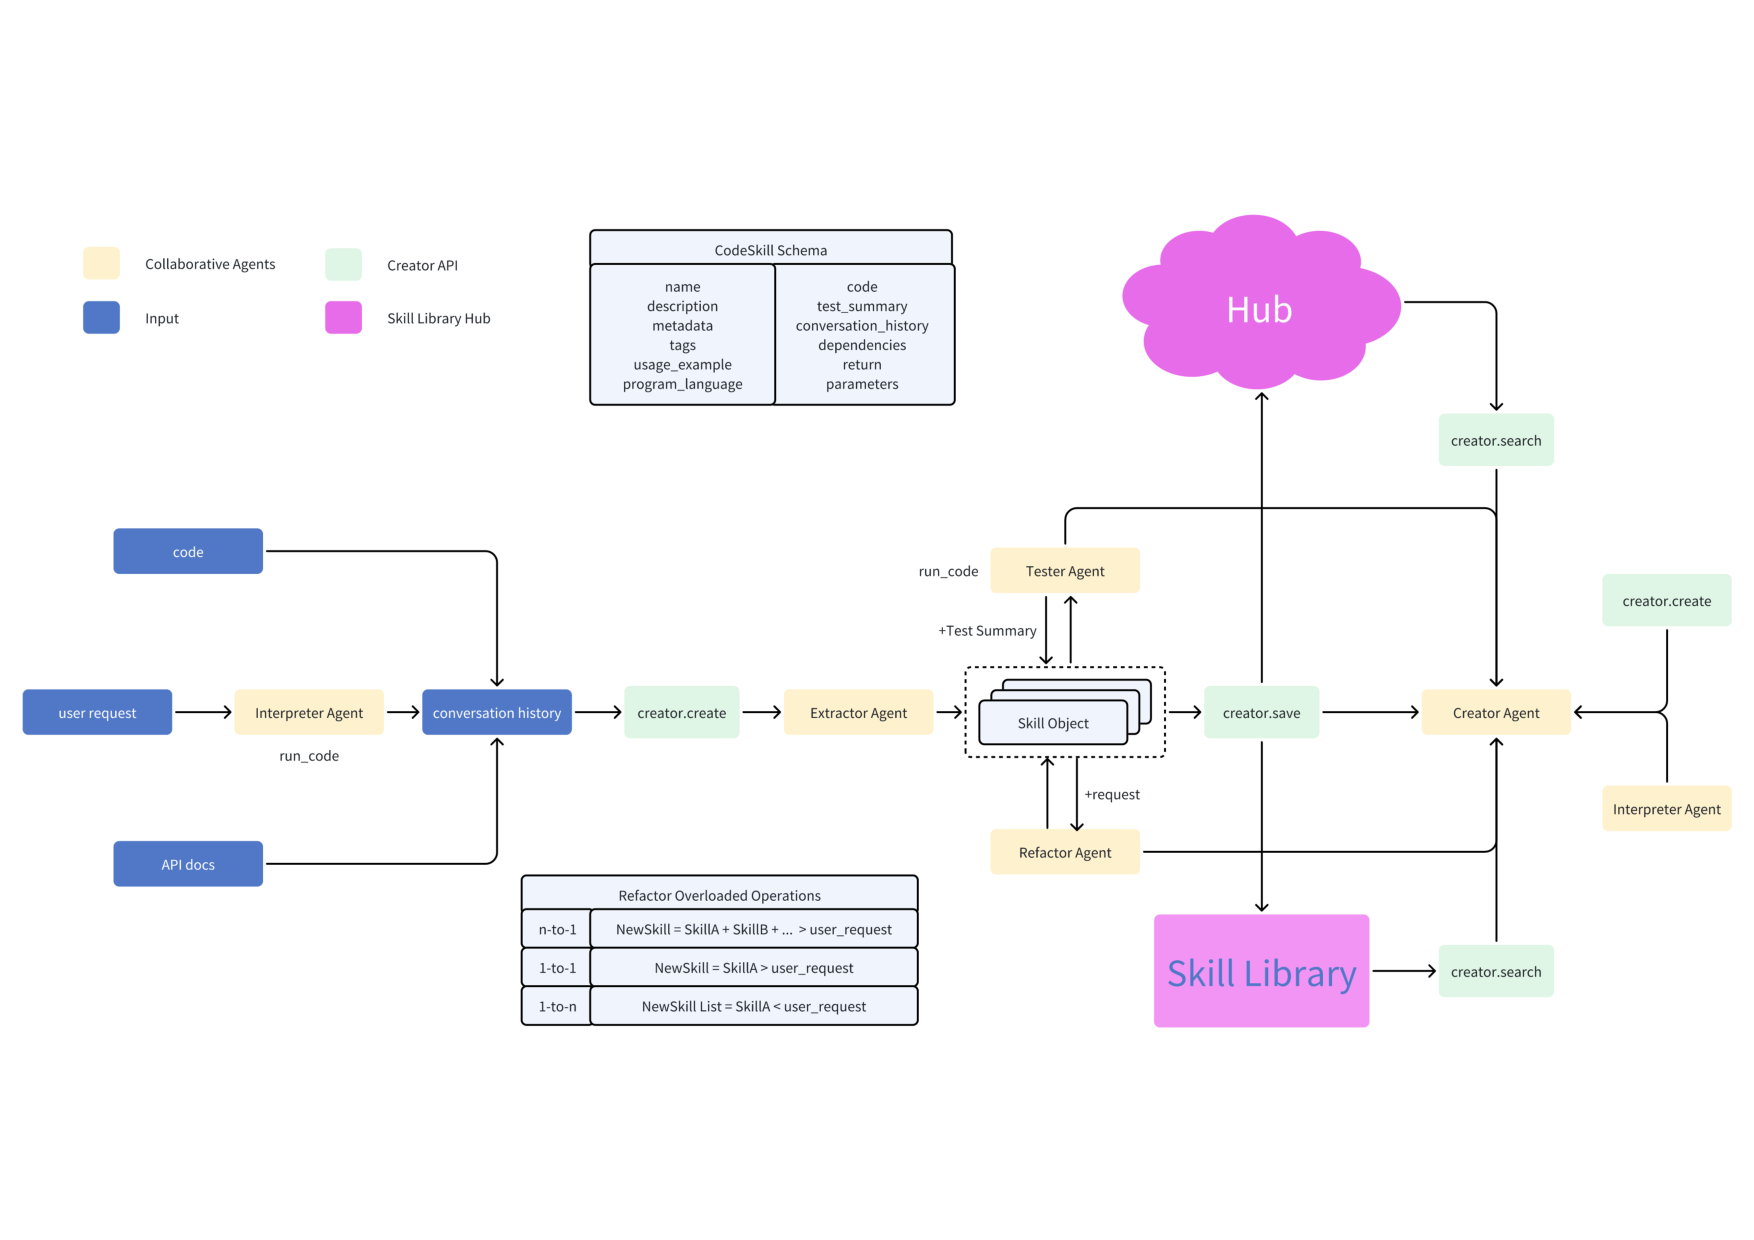
\includegraphics[width=1\textwidth]{./figures/creator_agents.pdf}
    \caption{\textbf{The Overview of Open-Creator Framework}}
    \label{fig:creator_agents}
\end{figure}
\section{Method}


Open-Creator is an integrated package, incorporating all functionalities of CREATOR agents along with additional features such as saving to local or remote skill libraries and performing RAG searches from the skill library. Open-Creator is composed of three main components: Creator API, Collaborative Agents, and Skill Library Hub.

\subsection{Creator API}

The Creator API is a pivotal component of Open-Creator, serving as an essential interface for both developers and researchers focused on AI agents and the AI agents themselves. Designed with an emphasis on simplicity and user-friendliness, the API primarily offers three critical functionalities:
\begin{enumerate}
    \item \textit{creator.create}: This function stands out for its versatility, enabling the generation of unified skill objects from a wide range of sources. Users can derive skill objects from dialogues between users and agents that have code interpreter tools, representing the problem-solving processes. Also, they can craft these objects directly from sources such as code files, API documentation, specific problem requirements, or even by utilizing existing skills.

    \item \textit{creator.save}: Once the skills are formulated, they require a reliable storage solution. This function offers the flexibility for users to save their skill objects in diverse formats. Be it locally or on cloud platforms like the Hugging Face Hub, users have the freedom to choose their preferred storage method.

    \item \textit{creator.search}: The retrieval process is streamlined with this function. It begins by transforming the structured skills into vectors. Following this, a semantic search mechanism is employed to ensure users can retrieve the top \( k \) skills, ideally suited for tackling new problems.
\end{enumerate}


\subsection{Collaborative Agents}

The Collaborative Agents encompasses five primary components:

\begin{enumerate}
    \item \textbf{Extractor Agent:} Responsible for converting existing problem-solving experiences (typically dialogues with a code interpreter), textual content, and documents into a unified skill object. The skill object encapsulates skill name, description, use cases, input-output parameters, associated dependencies, and code language. The code within the historical records is modularized and reorganized.
    
    \item \textbf{Interpreter Agent:} It leverages the open-source project, `open-interpreter` ~\cite{openinterpreter}, for prompt templates and code execution settings. The agent generates dialogue histories in the absence of known problem-solving procedures. Depending on execution results and user feedback, it preliminarily verifies the accuracy of results. The prompt templates of `open-interpreter` utilize thought chains and the rewoo framework. Initial approaches to user queries involve incremental planning and task decomposition, followed by execution and retrospective outlining of the next steps. The ReWOO ~\cite{xu2023rewoo} framework delineates the language model's inference process from external tool invocations, significantly reducing redundant prompts and computational requirements.
    
    \item \textbf{Tester Agent:} A variant of the interpreter agent, its primary role differs as it generates test cases and reports for stored skill objects. This evaluates their robustness and generalization performance, subsequently providing feedback to the interpreter for iterations.
    
    \item \textbf{Refactor Agent:} This agent facilitates modifications based on user demands. A technique involving operator overloading elegantly represents skill amalgamation, fine-tuning, and modularization of complex skills. Instead of repetitively restructuring extensive skill inputs, a mathematical operation-based approach simplifies the interface. Skill objects can be accumulated, and the resultant skill objects are appended with natural language using symbols > or <. For instance, "skillA + skillB > user\_request" represents the merging of two skills as per user demands. "SkillA < user\_request" illustrates the modularization of a complex skill based on user requirements. For skill fine-tuning, "skillA > user\_request" suffices.
    
    \item \textbf{Creator Agent:} This agent orchestrates the usage of the Creator API interfaces and coordinates the operations of the above four agents in response to user queries and intents. It uses the search interface to retrieve relevant skills for problem-solving. If the retrieved skills are inadequate, it employs the create interface to devise a new solution, followed by the save interface to persist the new skill. It inherently supports direct operations on API interfaces and dispatches responses across various agents. The agent also employs overloaded operators for skill iterative updates and refactoring.
\end{enumerate}

The Agents are developed on the langchain ~\cite{langchain} platform and are optimized with LLM cache. They are progressively designed to support diverse open-source or proprietary API-based LLMs.  Figure ~\ref{fig:creator_agents} aptly depicts their interrelationships.

\subsection{Skill Library Hub}

The Skill Library focuses on the persistent storage of skills. It employs a directory structure where each skill is stored in its named subfolder. Additionally, the advantages of the Hugging Face Hub community are harnessed to allow users to upload their private skill libraries to the cloud.

After users craft a skill, they have the option to save it on the cloud by providing a Hugging Face `repo\_id`. If the user hasn't established a repository, one is automatically forked from our pre-defined template. Following the fork, the user's skill is uploaded. To access skills from others' libraries, users need only supply the public repo\_id and the designated skill directory name for downloading locally. After downloading, the search index is auto-updated to include the new skill. With the community's growth around the skill library, we've also introduced cloud-based searching, making it easier to tap into collective community insights.

% \input{sections/4-experiments}
% \input{sections/5-discussions}
% \input{sections/6-conclusion}
\section{Acknowledgements}

We extend our heartfelt appreciation to Killian Lucas, the author of open-interpreter. We are also immensely grateful to the Discord community members, including warjiang, leonidas, AJ Ram, Papillon, minjunes, localman, jofus, Satake, oliveR, piotr, Grindelwald, Nico, MyRealNameIsTim, Pablo Vazquez, and jbexta, for their extensive discussions on the skill library and invaluable feedback. Their collective wisdom greatly enriched our work.

\newpage
%Bibliography
\bibliographystyle{unsrt}
\bibliography{references}  


\end{document}
